
\newcolumntype{Y}{>{\raggedright\arraybackslash}X}  %
\newcolumntype{C}{>{\centering\arraybackslash}X}    %

\newcommand{\abbrcite}[2]{%
  \mbox{#1\cite{#2}}\xspace}

\newcommand{\TBitemsep}{}

\begin{table}[tb]
  \caption{Summary of existing cyber-offense tools and their evaluation environment}
  \label{tab:attack_taxonomy}

  {\scriptsize %
  \setlength{\tabcolsep}{1pt} %
  \renewcommand\arraystretch{0.9}             %
  \centering
  \begin{tabularx}{\columnwidth}{@{}YCCCC@{}}
    \toprule
    \textbf{Evaluation environment}
      & \multicolumn{2}{c}{\textbf{Non‑LLM}}
      & \multicolumn{2}{c}{\textbf{LLM}} \\
    \cmidrule(lr){2-3}\cmidrule(lr){4-5}
      & Manual & Automated & Semi‑auto & Automated \\
    \midrule

    Single‑stage Single‑host 
\includegraphics[width=1.5cm]{figures/background/stages/single.png}&
      \abbrcite{MSF}{metasploit}\TBitemsep
      \abbrcite{NM}{nmap}\TBitemsep
      \abbrcite{HC}{hashcat} & – &
      \abbrcite{PT}{pentestgpt}\TBitemsep
      \abbrcite{CB}{zhang2024cybench} &
      \abbrcite{GP}{happe2023getting}\TBitemsep
      \abbrcite{YL}{yang2023language}\TBitemsep
      \abbrcite{IC}{intercode_ctf}\TBitemsep
      \abbrcite{FT}{fang2024teams}\TBitemsep
      \abbrcite{SH}{shao2024empirical} \\

    \midrule
    Multistage Single‑host 
\includegraphics[width=2cm]{figures/background/stages/multi_stage.png} &
      \abbrcite{MSF}{metasploit} &
      \abbrcite{CD}{caldera} &
      \abbrcite{PT}{pentestgpt}\TBitemsep
      \abbrcite{CB}{zhang2024cybench}\TBitemsep
      \abbrcite{AA}{xu2024autoattacker}\TBitemsep
      \abbrcite{AP}{al2025pentest} &
      \abbrcite{NY}{shao2024nyu_ctf}\TBitemsep
      \abbrcite{CA}{mayoral2025cai}\TBitemsep
      \abbrcite{CS}{cyberseceval3}\TBitemsep
      \abbrcite{O1}{o1systemcard}\TBitemsep
      \abbrcite{CB}{zhang2024cybench}\TBitemsep
      \abbrcite{AT}{anthropic_AISI}\TBitemsep
      \abbrcite{VB}{kong2025vulnbot} \\

    \midrule
    Multistage Multi‑host 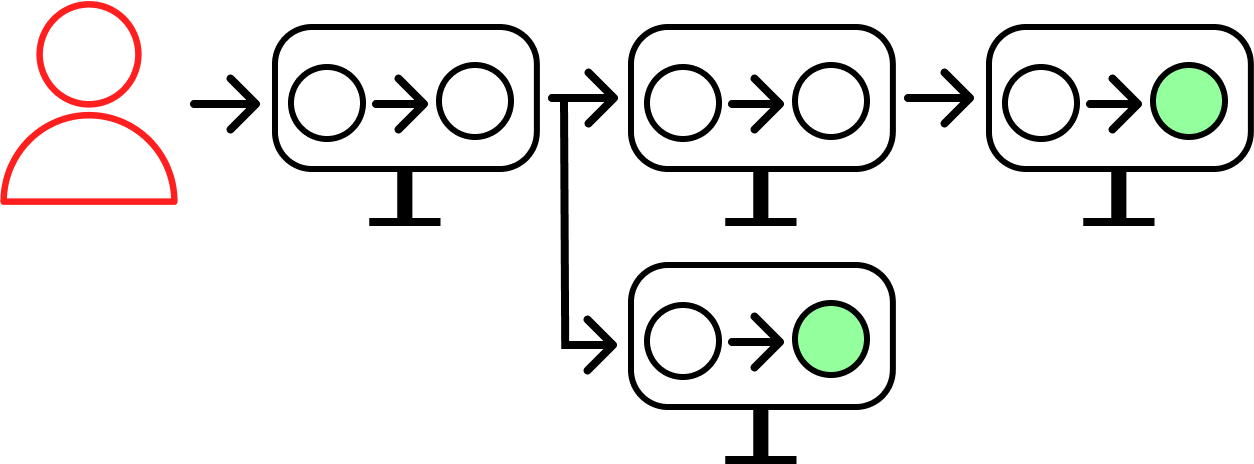
\includegraphics[width=3cm]{figures/background/stages/multi_host.png} &
      \abbrcite{MSF}{metasploit} &
      \abbrcite{CD}{caldera}\TBitemsep
      \abbrcite{LR}{holm2022lore}\TBitemsep
      \abbrcite{HR}{enoch2020harmer}\TBitemsep
      \abbrcite{CY}{yoo2020cyber}\TBitemsep
      \abbrcite{AJ}{ajmal2021offensive}\TBitemsep
      \abbrcite{SV}{sved_tool}\TBitemsep
      \abbrcite{HP}{Hu2020AutoPentestDRL}\TBitemsep
      \abbrcite{DE}{DeepExploit} &
      – &
      \sys\ \newline
      \abbrcite{OC}{kouremetis2025occult}\footnotemark\TBitemsep
      \\
    \midrule
     & Legend  &  
\includegraphics[width=3cm]{figures/background/stages/legend.png} &
  \end{tabularx}
  }%
\end{table}

\footnotetext{The MITRE OCCULT is a framework to understand the cyber security risks of LLMs.
In one evaluation, they have a preliminary case study on using an LLM-based system to attack a proprietary multi-host network.
Later, we evaluate \sysNoActions, a similar approach to the case study, on \benchmark and show that LLMs fail to even partially succeed in any environment.}
